%%%%%%%%%%%%%%%%%%%%%%%%%%%%%%%%%%%%%%%%%%%%%%%%%%%%%%%%%%%%%%%%%%%%%%%%%%%%%%%
% APPENDIX X: Milgrom & Roberts – Complementarities and Organization
% The Formal Foundations of Supermodularity and Strategic Complementarity
%%%%%%%%%%%%%%%%%%%%%%%%%%%%%%%%%%%%%%%%%%%%%%%%%%%%%%%%%%%%%%%%%%%%%%%%%%%%%%%
% Category: LIT
% Language: English
%%%%%%%%%%%%%%%%%%%%%%%%%%%%%%%%%%%%%%%%%%%%%%%%%%%%%%%%%%%%%%%%%%%%%%%%%%%%%%%

% =============================================================================
\begin{tcolorbox}[colback=blue!5!white, colframe=blue!75!black,
    title=Quick Reference: Appendix MIL]
\textbf{Appendix:} MIL (LIT)

\textbf{Core Question:} What are the key research findings in this literature domain?

\textbf{Key Concepts:}
\begin{itemize}[nosep]
\item Literature synthesis and integration
\item Framework application and validation
\item Cross-domain connections
\end{itemize}

\textbf{Cross-References:} See Chapter linkage below
\end{tcolorbox}


\begin{abstract}
This appendix provides a systematic review and integration of key research findings
in the LIT domain. It synthesizes literature relevant to the Evidence-Based
Framework (EBF) and identifies connections to the 10C CORE architecture.
\end{abstract}

\section{The Fundamental Question}
\label{sec:mil-fundamental}
%%%%%%%%%%%%%%%%%%%%%%%%%%%%%%%%%%%%%%%%%%%%%%%%%%%%%%%%%%%%%%%%%%%%%%%%%%%%%%%

\begin{tcolorbox}[
    colback=red!5!white,
    colframe=red!75!black,
    title={\textbf{Fundamental Question}}
]
\textbf{How does unknown integrate with and contribute to the
Evidence-Based Framework for understanding behavioral outcomes?}

This appendix addresses the core challenge of formalizing behavioral principles
within a rigorous theoretical framework while maintaining practical applicability.
\end{tcolorbox}


\section{Milgrom \& Roberts: The Formal Theory of Complementarities}
\label{app:milgrom-roberts}

%==============================================================================
% PART 0: INTEGRATION OVERVIEW
%==============================================================================
\subsection{Framework Integration Map}

This appendix demonstrates how the research program of Paul Milgrom and John Roberts 
provides the \textbf{formal mathematical foundations} for the complementarity structure 
$C$ in the $(C, \Psi, C^*, K, Q)$ framework. Their work on supermodularity, strategic 
complementarity, and organizational economics establishes when and why $C_{ij} > 0$ 
matters for equilibrium existence, comparative statics, and optimal organizational design.

\begin{center}
\renewcommand{\arraystretch}{1.4}
\begin{tabular}{|l|l|l|}
\hline
\textbf{Framework Element} & \textbf{M/R Contribution} & \textbf{Key Papers} \\
\hline
$C_{ij} > 0$ (Complementarity) & Supermodularity theory & Topkis 1978, M\&R 1990 \\
$C^*$ Existence \& Uniqueness & Lattice-theoretic methods & M\&R 1990, Vives 1990 \\
$\partial C^* / \partial \Psi$ & Monotone comparative statics & Milgrom \& Shannon 1994 \\
Organizational $C$ & Modern manufacturing & M\&R 1990, 1995 \\
Strategic $C_{ij}$ & Game-theoretic foundations & M\&R 1990, Bulow et al. 1985 \\
$C^*$ as system & Complementary practices & Ichniowski et al. 1997 \\
\hline
\end{tabular}
\end{center}

\paragraph{Milgrom \& Roberts' Unique Role.}
While other contributors provide empirical evidence for complementarities (Bloom: 
management; Stiglitz: information), Milgrom \& Roberts uniquely establish:
\begin{enumerate}
    \item \textbf{Mathematical formalization} of what ``complementarity'' means
    \item \textbf{Existence theorems} for equilibria in complementary systems
    \item \textbf{Comparative statics} that are robust and monotone
    \item \textbf{Organizational implications} of complementarity structures
    \item \textbf{Why systems matter}: practices must be adopted together
\end{enumerate}

%==============================================================================
% PART I: SUPERMODULARITY – THE MATHEMATICS OF C_{ij} > 0
%==============================================================================
\subsection{Part I: Supermodularity – The Mathematics of $C_{ij} > 0$}

\subsubsection{Theoretical Foundation}

The framework's complementarity condition $C_{ij} > 0$ is formalized through 
supermodularity:

\begin{equation}
\boxed{
f \text{ is supermodular} \quad \Leftrightarrow \quad 
\frac{\partial^2 f}{\partial x_i \partial x_j} \geq 0 \quad \forall i \neq j
}
\label{eq:mr-supermodular}
\end{equation}

\paragraph{Equivalent Definition (Lattice-Theoretic).}
For any $x, y$ in the domain:
\begin{equation}
f(x \vee y) + f(x \wedge y) \geq f(x) + f(y)
\end{equation}
where $x \vee y = \max(x,y)$ and $x \wedge y = \min(x,y)$ component-wise.

\subsubsection{Why Supermodularity Matters}

Supermodularity provides:
\begin{enumerate}
    \item \textbf{Existence:} Equilibria exist under weak conditions
    \item \textbf{Monotonicity:} Equilibria respond monotonically to parameters
    \item \textbf{Extremal equilibria:} Largest and smallest equilibria always exist
    \item \textbf{Comparative statics:} Parameter increases raise equilibrium values
\end{enumerate}

\subsubsection{Framework Translation}

The framework's $C$ matrix is the Hessian of the value function:
\begin{equation}
C_{ij} = \frac{\partial^2 V}{\partial x_i \partial x_j}
\end{equation}

When $V$ is supermodular ($C_{ij} \geq 0$ for all $i \neq j$):
\begin{itemize}
    \item Activities $x_i$ and $x_j$ are \textbf{complements}
    \item Increasing $x_i$ raises the marginal return to $x_j$
    \item Optimal choices are \textbf{positively correlated}
\end{itemize}

%==============================================================================
% PART II: STRATEGIC COMPLEMENTARITY IN GAMES
%==============================================================================
\subsection{Part II: Strategic Complementarity in Games}

\subsubsection{Theoretical Foundation}

Milgrom \& Roberts (1990) extend supermodularity to games:

\begin{equation}
\boxed{
\frac{\partial^2 u_i}{\partial a_i \partial a_j} > 0 \quad \Rightarrow \quad 
\text{Strategic complements}
}
\label{eq:mr-strategic}
\end{equation}

When my action and your action are strategic complements, my best response 
is increasing in your action.

\subsubsection{Supermodular Games}

A game is \textbf{supermodular} if:
\begin{enumerate}
    \item Action spaces are lattices
    \item Payoff functions are supermodular in own action
    \item Payoffs have increasing differences in $(a_i, a_{-i})$
\end{enumerate}

\paragraph{Key Results for Supermodular Games.}
\begin{itemize}
    \item Pure strategy Nash equilibrium \textbf{always exists}
    \item The set of equilibria forms a complete lattice
    \item \textbf{Largest} and \textbf{smallest} equilibria exist
    \item Best response dynamics converge (from extremes)
\end{itemize}

\subsubsection{Framework Translation}

$C^*$ in the framework is Nash equilibrium in a supermodular game:
\begin{equation}
C^* = \{a^* : a^*_i \in BR_i(a^*_{-i}) \quad \forall i\}
\end{equation}

When $C_{ij} > 0$ (strategic complements):
\begin{itemize}
    \item $C^*$ exists (existence theorem)
    \item Multiple $C^*$ possible but ordered (lattice structure)
    \item Coordination on high vs. low equilibrium depends on $\Psi$
\end{itemize}

\subsubsection{Strategic Complements vs. Substitutes}

\begin{center}
\renewcommand{\arraystretch}{1.3}
\begin{tabular}{|l|c|c|}
\hline
& \textbf{Complements} ($C_{ij} > 0$) & \textbf{Substitutes} ($C_{ij} < 0$) \\
\hline
Best response & Increasing & Decreasing \\
Equilibrium & Multiple possible & Unique (typically) \\
Coordination & Critical & Less important \\
Examples & Network effects, arms races & Cournot competition \\
\hline
\end{tabular}
\end{center}

%==============================================================================
% PART III: MONOTONE COMPARATIVE STATICS
%==============================================================================
\subsection{Part III: Monotone Comparative Statics}

\subsubsection{Theoretical Foundation}

Milgrom \& Shannon (1994) establish that supermodularity yields robust 
comparative statics:

\begin{equation}
\boxed{
\frac{\partial^2 f}{\partial x \partial \theta} \geq 0 \quad \Rightarrow \quad 
x^*(\theta) \text{ is increasing in } \theta
}
\label{eq:mr-mcs}
\end{equation}

\paragraph{The Single Crossing Property.}
Even without supermodularity, if $f$ satisfies single crossing in $(x, \theta)$:
\begin{equation}
f(x', \theta') - f(x, \theta') \geq 0 \quad \Rightarrow \quad 
f(x', \theta'') - f(x, \theta'') \geq 0 \quad \text{for } \theta'' > \theta'
\end{equation}
then $x^*(\theta)$ is monotone.

\subsubsection{Framework Translation}

This provides the foundation for $\partial C^* / \partial \Psi$:
\begin{equation}
\frac{\partial^2 V}{\partial C \partial \Psi} \geq 0 \quad \Rightarrow \quad 
C^*(\Psi) \text{ is increasing in } \Psi
\end{equation}

\paragraph{Implications.}
\begin{itemize}
    \item Policy changes ($\Delta \Psi$) have \textbf{predictable direction} on $C^*$
    \item No need to solve for equilibrium explicitly
    \item Comparative statics are \textbf{robust} to functional form
\end{itemize}

\subsubsection{Application: Policy Analysis}

When analyzing policy intervention $\Psi \to \Psi'$:
\begin{enumerate}
    \item Check if $V$ has increasing differences in $(C, \Psi)$
    \item If yes: $\Psi' > \Psi \Rightarrow C^*(\Psi') \geq C^*(\Psi)$
    \item Direction of effect known without computing equilibrium
\end{enumerate}

%==============================================================================
% PART IV: MODERN MANUFACTURING AND ORGANIZATIONAL COMPLEMENTARITIES
%==============================================================================
\subsection{Part IV: Modern Manufacturing and Organizational Complementarities}

\subsubsection{Theoretical Foundation}

Milgrom \& Roberts (1990, 1995) show that modern manufacturing involves 
\textbf{systems of complementary practices}:

\begin{equation}
\boxed{
\frac{\partial^2 \Pi}{\partial M_i \partial M_j} > 0 \quad \forall i, j \in \text{Modern Practices}
}
\label{eq:mr-manufacturing}
\end{equation}

\subsubsection{The Modern Manufacturing System}

Complementary practices include:

\begin{center}
\renewcommand{\arraystretch}{1.3}
\begin{tabular}{|l|l|}
\hline
\textbf{Practice Category} & \textbf{Specific Elements} \\
\hline
Production & Flexible manufacturing, small batches, low inventory \\
Quality & TQM, statistical process control, continuous improvement \\
Labor & Team production, worker training, broad task assignment \\
Supplier & Long-term relationships, JIT delivery, joint design \\
Technology & CAD/CAM, rapid prototyping, information systems \\
\hline
\end{tabular}
\end{center}

\paragraph{Key Insight: System, Not Components.}
The complementarities mean:
\begin{itemize}
    \item Adopting one practice \textbf{raises returns} to others
    \item Partial adoption is \textbf{worse than none or all}
    \item Firms cluster at \textbf{low} (traditional) or \textbf{high} (modern) configurations
    \item Transition requires \textbf{simultaneous} change
\end{itemize}

\subsubsection{Framework Translation}

This is the core insight for organizational $C^*$:
\begin{equation}
C^*_{org} \in \{C^*_{traditional}, C^*_{modern}\} \quad \text{with little in between}
\end{equation}

The ``stuck in the middle'' phenomenon: firms attempting partial modernization 
perform worse than either extreme.

\subsubsection{Empirical Validation}

Ichniowski, Shaw \& Prennushi (1997) confirm:
\begin{itemize}
    \item Steel mills using \textbf{all} innovative practices: +6.7\% productivity
    \item Mills using \textbf{some} practices: negligible or negative effect
    \item Complementarity is \textbf{empirically verified}
\end{itemize}

%==============================================================================
% PART V: COMPLEMENTARITIES IN INCENTIVES AND ORGANIZATION
%==============================================================================
\subsection{Part V: Complementarities in Incentives and Organization}

\subsubsection{Pay and Performance}

Milgrom \& Roberts (1995) analyze complementarities between:
\begin{itemize}
    \item Incentive pay and performance measurement
    \item Decentralization and information systems
    \item Training and job enrichment
\end{itemize}

\begin{equation}
\frac{\partial^2 \text{Performance}}{\partial \text{Incentive Pay} \times \partial \text{Measurement Quality}} > 0
\end{equation}

Incentive pay works only when performance is measurable.

\subsubsection{Influence Costs}

Milgrom (1988) and Milgrom \& Roberts (1988) introduce \textbf{influence costs}:
\begin{equation}
\text{Total Cost} = \text{Production Cost} + \text{Influence Cost}(\Psi_{org})
\end{equation}

Organizational design affects how much effort goes to productive vs. 
redistributive activities.

\paragraph{Framework Translation.}
$\Psi_{org}$ (organizational context) determines:
\begin{itemize}
    \item Whether incentives complement or conflict
    \item How much effort is ``wasted'' on influence
    \item Optimal centralization vs. decentralization
\end{itemize}

\subsubsection{The Economics of Organization}

Milgrom \& Roberts (1992) textbook synthesizes:
\begin{equation}
\text{Optimal Organization} = \arg\max_{org} V(org; \Psi) \quad \text{s.t. } C_{ij}(org) \text{ structure}
\end{equation}

Different $\Psi$ (technology, information, markets) call for different organizational $C^*$.

%==============================================================================
% PART VI: AUCTION THEORY AND MECHANISM DESIGN
%==============================================================================
\subsection{Part VI: Auction Theory and Market Design}

\subsubsection{Theoretical Foundations}

Milgrom's auction theory (Nobel 2020) applies complementarity to mechanism design:

\begin{equation}
\boxed{
\text{Auction design} = \text{Choose } \Psi_{mechanism} \text{ to achieve } C^*_{efficient}
}
\label{eq:mr-auction}
\end{equation}

\subsubsection{Complementarities Among Goods}

The \textbf{combinatorial auction problem}: when goods are complements, 
package bidding is essential:
\begin{equation}
v(A \cup B) > v(A) + v(B) \quad \Rightarrow \quad \text{Bundle bidding needed}
\end{equation}

\paragraph{Spectrum Auctions.}
Adjacent spectrum licenses are complements:
\begin{itemize}
    \item Milgrom designed FCC spectrum auctions
    \item Simultaneous ascending auction allows package discovery
    \item Handles complementarities among licenses
\end{itemize}

\subsubsection{Framework Translation}

Auction design is $\Psi_{mechanism}$ design:
\begin{equation}
\Psi_{mechanism} \to C^*_{allocation} \to Q_{efficiency}
\end{equation}

The mechanism designer chooses rules ($\Psi$) to induce efficient equilibrium ($C^*$).

%==============================================================================
% PART VII: SYNTHESIS – THE MILGROM-ROBERTS EQUATIONS
%==============================================================================
\subsection{Part VII: Synthesis – The Milgrom-Roberts Equations}

\subsubsection{Complete Framework Translation}

\begin{center}
\renewcommand{\arraystretch}{1.5}
\begin{tabular}{|l|c|l|}
\hline
\textbf{M/R Finding} & \textbf{Equation} & \textbf{Framework Element} \\
\hline
Supermodularity & $\frac{\partial^2 f}{\partial x_i \partial x_j} \geq 0$ & Definition of $C_{ij} \geq 0$ \\
\hline
Equilibrium existence & Lattice $\Rightarrow \exists C^*$ & $C^*$ always exists \\
\hline
Multiple equilibria & $C^*_{low} \preceq C^*_{high}$ & Coordination problem \\
\hline
Monotone comp. statics & $\partial C^* / \partial \Psi \geq 0$ & Directional predictions \\
\hline
System complementarity & $C_{M_i, M_j} > 0$ all pairs & Practices adopted together \\
\hline
Stuck in middle & Partial adoption fails & $C^*$ is discrete \\
\hline
Influence costs & $\Psi_{org}$ affects waste & Organization matters \\
\hline
Combinatorial auctions & $v(A \cup B) > v(A) + v(B)$ & Package bidding \\
\hline
\end{tabular}
\end{center}

\subsubsection{Milgrom \& Roberts' Unique Contribution}

\textbf{Without Milgrom \& Roberts, the framework would:}
\begin{itemize}
    \item Lack formal definition of ``complementarity''
    \item Have no existence theorems for $C^*$
    \item Miss monotone comparative statics
    \item Not understand why practices cluster
    \item Lack tools for mechanism design
\end{itemize}

\textbf{With Milgrom \& Roberts, the framework gains:}
\begin{itemize}
    \item Rigorous mathematics: supermodularity, lattice theory
    \item Existence guarantees: $C^*$ exists under complementarity
    \item Robust predictions: monotone comparative statics
    \item Organizational theory: why systems matter
    \item Design tools: auction and mechanism design
\end{itemize}

%==============================================================================
% PART VIII: COMPLETE PAPER DOCUMENTATION
%==============================================================================
\subsection{Part VIII: Complete Paper Documentation}

%--- FOUNDATIONAL THEORY ---
\subsubsection{Foundational Supermodularity Theory}

\paragraph{Paper 1: Topkis (1978)}

``Minimizing a Submodular Function on a Lattice.''
\textit{Operations Research}, 26(2), 305--321.

\textbf{Summary.}
Establishes mathematical foundations of supermodularity on lattices. 
Proves key theorems on optimization of supermodular functions.

\textbf{Framework Translation.}
Provides the mathematical toolkit:
\begin{equation}
\arg\max_x f(x) \text{ is a lattice when } f \text{ is supermodular}
\end{equation}

\paragraph{Paper 2: Topkis (1998)}

\textit{Supermodularity and Complementarity.}
Princeton University Press.

\textbf{Summary.}
Definitive textbook treatment of supermodularity theory with economic applications.

\textbf{Framework Translation.}
Complete mathematical foundations for $C_{ij}$ analysis.

\paragraph{Paper 3: Milgrom \& Roberts (1990)}

``Rationalizability, Learning, and Equilibrium in Games with Strategic Complementarities.''
\textit{Econometrica}, 58(6), 1255--1277.

\textbf{Summary.}
Foundational paper applying supermodularity to games. Shows equilibrium exists, 
extremal equilibria exist, and dynamics converge.

\textbf{Framework Translation.}
\begin{equation}
C_{ij}^{strategic} > 0 \Rightarrow C^* \text{ exists and has lattice structure}
\end{equation}

\textbf{Key Finding.}
Most influential paper on strategic complementarity. 3,000+ citations.

\paragraph{Paper 4: Vives (1990)}

``Nash Equilibrium with Strategic Complementarities.''
\textit{Journal of Mathematical Economics}, 19(3), 305--321.

\textbf{Summary.}
Parallel development of supermodular game theory. Establishes similar results 
with different proof techniques.

\textbf{Framework Translation.}
Independent confirmation of $C^*$ existence under complementarity.

\paragraph{Paper 5: Milgrom \& Shannon (1994)}

``Monotone Comparative Statics.''
\textit{Econometrica}, 62(1), 157--180.

\textbf{Summary.}
Establishes conditions for comparative statics without calculus. 
Single crossing property as key condition.

\textbf{Framework Translation.}
\begin{equation}
\frac{\partial C^*}{\partial \Psi} \geq 0 \quad \text{under single crossing}
\end{equation}
Direction of policy effects known without solving model.

\textbf{Key Finding.}
Revolutionized comparative statics methodology. 2,500+ citations.

%--- ORGANIZATIONAL ECONOMICS ---
\subsubsection{Organizational Economics}

\paragraph{Paper 6: Milgrom \& Roberts (1990)}

``The Economics of Modern Manufacturing: Technology, Strategy, and Organization.''
\textit{American Economic Review}, 80(3), 511--528.

\textbf{Summary.}
Shows modern manufacturing practices are complements. Firms optimally adopt 
all or none, explaining discrete organizational forms.

\textbf{Framework Translation.}
\begin{equation}
C^*_{org} \in \{C^*_{traditional}, C^*_{modern}\}
\end{equation}
Organizational coherence is discrete, not continuous.

\textbf{Key Finding.}
Launched literature on practice complementarity. 4,000+ citations.

\paragraph{Paper 7: Milgrom \& Roberts (1995)}

``Complementarities and Fit: Strategy, Structure, and Organizational Change in Manufacturing.''
\textit{Journal of Accounting and Economics}, 19(2-3), 179--208.

\textbf{Summary.}
Extends complementarity analysis to strategy-structure fit. 
Analyzes Lincoln Electric as case study.

\textbf{Framework Translation.}
\begin{equation}
K_{org} = \text{Alignment}(Strategy, Structure, Practices)
\end{equation}
Coherence requires fit across multiple dimensions.

\paragraph{Paper 8: Milgrom \& Roberts (1992)}

\textit{Economics, Organization and Management.}
Prentice Hall.

\textbf{Summary.}
Comprehensive textbook applying economic theory to organizational design. 
Covers incentives, coordination, boundaries.

\textbf{Framework Translation.}
Organizational $C^*$ depends on:
\begin{itemize}
    \item Technology ($\Psi_{tech}$)
    \item Information ($\Psi_K$)
    \item Incentives ($\Psi_{incentive}$)
\end{itemize}

\paragraph{Paper 9: Milgrom (1988)}

``Employment Contracts, Influence Activities, and Efficient Organization Design.''
\textit{Journal of Political Economy}, 96(1), 42--60.

\textbf{Summary.}
Introduces influence costs. Shows organizational design affects how much 
effort goes to productive vs. redistributive activities.

\textbf{Framework Translation.}
\begin{equation}
Q_{net} = Q_{gross} - \text{Influence Costs}(\Psi_{org})
\end{equation}

\paragraph{Paper 10: Milgrom \& Roberts (1988)}

``An Economic Approach to Influence Activities in Organizations.''
\textit{American Journal of Sociology}, 94(Supplement), S154--S179.

\textbf{Summary.}
Develops theory of influence activities and organizational responses 
(bureaucratic rules, centralization).

\textbf{Framework Translation.}
$\Psi_{org}$ design trades off:
\begin{itemize}
    \item Flexibility vs. influence costs
    \item Decentralization vs. coordination
\end{itemize}

%--- EMPIRICAL VALIDATION ---
\subsubsection{Empirical Validation}

\paragraph{Paper 11: Ichniowski, Shaw \& Prennushi (1997)}

``The Effects of Human Resource Management Practices on Productivity: A Study of Steel Finishing Lines.''
\textit{American Economic Review}, 87(3), 291--313.

\textbf{Summary.}
Tests complementarity hypothesis in steel industry. Finds systems of practices 
matter; individual practices don't.

\textbf{Framework Translation.}
\begin{equation}
\Delta Q = f(\text{System}) \neq \sum_i f_i(\text{Practice}_i)
\end{equation}
Empirical validation of complementarity.

\textbf{Key Finding.}
Definitive empirical test of M\&R theory. 3,500+ citations.

\paragraph{Paper 12: Brynjolfsson \& Milgrom (2013)}

``Complementarity in Organizations.''
\textit{Handbook of Organizational Economics}, 11--55.

\textbf{Summary.}
Comprehensive survey of complementarity in organizations. Reviews theory, 
evidence, and applications.

\textbf{Framework Translation.}
State-of-the-art synthesis of organizational $C_{ij}$.

%--- AUCTION THEORY AND MECHANISM DESIGN ---
\subsubsection{Auction Theory and Mechanism Design}

\paragraph{Paper 13: Milgrom \& Weber (1982)}

``A Theory of Auctions and Competitive Bidding.''
\textit{Econometrica}, 50(5), 1089--1122.

\textbf{Summary.}
Foundational auction theory paper. Analyzes common value auctions, 
winner's curse, and revenue equivalence.

\textbf{Framework Translation.}
Auctions as $\Psi_{mechanism}$ that induces $C^*_{allocation}$.

\textbf{Key Finding.}
Most cited auction theory paper. Foundation for Nobel Prize.

\paragraph{Paper 14: Milgrom (2004)}

\textit{Putting Auction Theory to Work.}
Cambridge University Press.

\textbf{Summary.}
Applies auction theory to practical design problems: spectrum, electricity, 
procurement.

\textbf{Framework Translation.}
$\Psi_{mechanism}$ design for real markets with complementarities.

\paragraph{Paper 15: Milgrom (2017)}

\textit{Discovering Prices: Auction Design in Markets with Complex Constraints.}
Columbia University Press.

\textbf{Summary.}
Latest developments in auction design. Handles complex complementarities 
and substitutabilities.

\textbf{Framework Translation.}
\begin{equation}
\text{Design } \Psi \text{ for } C^* \text{ when } C_{ij} \text{ varies across goods}
\end{equation}

%--- INFORMATION AND COMMUNICATION ---
\subsubsection{Information and Communication}

\paragraph{Paper 16: Milgrom \& Roberts (1986)}

``Relying on the Information of Interested Parties.''
\textit{RAND Journal of Economics}, 17(1), 18--32.

\textbf{Summary.}
When can decision-makers rely on information from biased sources? 
Shows competition among informants can reveal truth.

\textbf{Framework Translation.}
$\Psi_K$ can be improved through strategic information transmission.

\paragraph{Paper 17: Milgrom \& Roberts (1986)}

``Price and Advertising Signals of Product Quality.''
\textit{Journal of Political Economy}, 94(4), 796--821.

\textbf{Summary.}
Price and advertising jointly signal quality. Analyzes equilibrium 
signaling when multiple signals available.

\textbf{Framework Translation.}
Signals are complements:
\begin{equation}
C_{price, advertising}^{signal} > 0
\end{equation}

\paragraph{Paper 18: Milgrom (1981)}

``Good News and Bad News: Representation Theorems and Applications.''
\textit{Bell Journal of Economics}, 12(2), 380--391.

\textbf{Summary.}
When does more information lead to higher or lower expected values? 
Establishes conditions for ``good news'' processes.

\textbf{Framework Translation.}
$\Delta \Psi_K$ effects depend on information structure.

%--- ENTRY AND COMPETITION ---
\subsubsection{Entry and Competition}

\paragraph{Paper 19: Milgrom \& Roberts (1982)}

``Limit Pricing and Entry under Incomplete Information: An Equilibrium Analysis.''
\textit{Econometrica}, 50(2), 443--459.

\textbf{Summary.}
Incumbent pricing signals costs to potential entrants. Analyzes 
separating and pooling equilibria.

\textbf{Framework Translation.}
Entry deterrence as $C^*$ in signaling game under $\Psi_K$ asymmetry.

\paragraph{Paper 20: Milgrom \& Roberts (1982)}

``Predation, Reputation, and Entry Deterrence.''
\textit{Journal of Economic Theory}, 27(2), 280--312.

\textbf{Summary.}
Rational predation can occur to build reputation. Chain-store paradox resolved.

\textbf{Framework Translation.}
$C^*$ over time: current actions affect future $\Psi$ (reputation).


%%%%%%%%%%%%%%%%%%%%%%%%%%%%%%%%%%%%%%%%%%%%%%%%%%%%%%%%%%%%%%%%%%%%%%%%%%%%%%%
% PART IX: THE MODERN FIRM (ROBERTS 2004)
% Applied Complementarity in Organizational Design
%%%%%%%%%%%%%%%%%%%%%%%%%%%%%%%%%%%%%%%%%%%%%%%%%%%%%%%%%%%%%%%%%%%%%%%%%%%%%%%
\subsection{Part IX: The Modern Firm (Roberts 2004) -- Applied Complementarity}
\label{sec:modern-firm}

While the academic papers of Milgrom \& Roberts establish the mathematical foundations,
Roberts' book \textit{The Modern Firm: Organizational Design for Performance and Growth}
(Oxford University Press, 2004) provides the \textbf{applied translation} of complementarity
theory to practical organizational design. This section documents the key concepts and
their integration into the EBF framework.

\subsubsection{Book Overview and Core Thesis}

\paragraph{Central Argument.}
Roberts (2004, p. ix) states the core thesis directly:
\begin{quote}
``The most fundamental responsibilities of general managers are setting strategy 
and designing the organization to implement it. [...] This book attempts to show 
how economics can contribute [...] to organizational design.''
\end{quote}

The book applies complementarity theory to explain why certain organizational 
configurations succeed while others fail. The key insight: \textbf{fit} between 
environment, strategy, and organization determines performance.

\paragraph{Chapter Structure.}
\begin{center}
\renewcommand{\arraystretch}{1.3}
\begin{tabular}{|c|l|l|}
\hline
\textbf{Ch.} & \textbf{Title} & \textbf{EBF Relevance} \\
\hline
1 & Strategy and Organization & Environment-Strategy-Org Fit \\
2 & Key Concepts for Organization Design & Complementarity Definition \\
3 & The Nature and Purpose of the Firm & Firm Boundaries \\
4 & Motivation in the Modern Firm & Incentives $\leftrightarrow$ PARC \\
5 & Organizing for Performance & PARC Implementation \\
6 & Organizing for Growth and Innovation & Dynamic Capabilities \\
7 & Creating the Modern Firm & Leadership \& Change \\
\hline
\end{tabular}
\end{center}

\subsubsection{The PARC Framework}
\label{sec:parc}

Roberts organizes the elements of organizational design into four interrelated 
categories. While not using the acronym ``PARC'' explicitly, the framework is 
clearly structured around these four dimensions.

\paragraph{Definition (PARC Components).}
\begin{enumerate}
    \item \textbf{People (P)}: The human capital of the organization
    \begin{itemize}
        \item Skills, capabilities, and competencies
        \item Mindsets and mental models
        \item Networks and relationships
        \item Selection, development, and retention
    \end{itemize}
    
    \item \textbf{Architecture (A)}: The formal structure of the organization
    \begin{itemize}
        \item Organizational structure (divisions, functions, matrix)
        \item Authority and decision rights allocation
        \item Information systems and flows
        \item Physical and technological infrastructure
    \end{itemize}
    
    \item \textbf{Routines (R)}: The processes and practices
    \begin{itemize}
        \item Standard operating procedures
        \item Planning and budgeting processes
        \item Performance management systems
        \item Coordination mechanisms
    \end{itemize}
    
    \item \textbf{Culture (C)}: The informal organization
    \begin{itemize}
        \item Shared values and beliefs
        \item Norms of behavior
        \item Trust and social capital
        \item Identity and meaning
    \end{itemize}
\end{enumerate}

\paragraph{PARC Complementarity Matrix.}
The four PARC elements are not independent---they must be \textbf{mutually reinforcing}:

\begin{center}
\renewcommand{\arraystretch}{1.4}
\begin{tabular}{|c|c|c|c|c|}
\hline
$\gamma_{PARC}$ & \textbf{P} & \textbf{A} & \textbf{R} & \textbf{C} \\
\hline
\textbf{P} & -- & $\gamma_{PA}$ & $\gamma_{PR}$ & $\gamma_{PC}$ \\
\textbf{A} & $\gamma_{PA}$ & -- & $\gamma_{AR}$ & $\gamma_{AC}$ \\
\textbf{R} & $\gamma_{PR}$ & $\gamma_{AR}$ & -- & $\gamma_{RC}$ \\
\textbf{C} & $\gamma_{PC}$ & $\gamma_{AC}$ & $\gamma_{RC}$ & -- \\
\hline
\end{tabular}
\end{center}

\begin{itemize}
    \item $\gamma_{PA}$: People need enabling architecture (skills $\times$ authority)
    \item $\gamma_{PR}$: People need supporting routines (capabilities $\times$ processes)
    \item $\gamma_{PC}$: People need cultural alignment (mindsets $\times$ values)
    \item $\gamma_{AR}$: Architecture needs process fit (structure $\times$ systems)
    \item $\gamma_{AC}$: Architecture needs cultural acceptance (technology $\times$ norms)
    \item $\gamma_{RC}$: Routines need cultural support (practices $\times$ beliefs)
\end{itemize}

\subsubsection{Environment--Strategy--Organization Fit}

\paragraph{The Fit Concept.}
Roberts (2004, Ch. 1) emphasizes that performance depends on \textbf{alignment}
among three elements:

\begin{center}
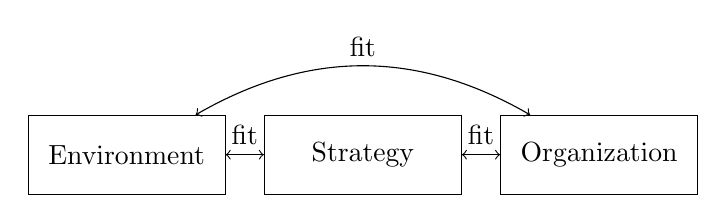
\begin{tikzpicture}[node distance=3cm]
\node (E) [draw, rectangle, minimum width=2.5cm, minimum height=1cm] {Environment};
\node (S) [draw, rectangle, minimum width=2.5cm, minimum height=1cm, right of=E] {Strategy};
\node (O) [draw, rectangle, minimum width=2.5cm, minimum height=1cm, right of=S] {Organization};
\draw[<->] (E) -- (S) node[midway, above] {fit};
\draw[<->] (S) -- (O) node[midway, above] {fit};
\draw[<->, bend left=30] (E) to node[midway, above] {fit} (O);
\end{tikzpicture}
\end{center}

\paragraph{EBF Translation.}
This directly maps to our framework:
\begin{itemize}
    \item \textbf{Environment} $\rightarrow$ Context $\Psi$ (CORE-WHEN)
    \item \textbf{Strategy} $\rightarrow$ Objectives, preferences within $U$
    \item \textbf{Organization} $\rightarrow$ PARC configuration
    \item \textbf{Fit} $\rightarrow$ Coherence Index $K$
\end{itemize}

Roberts' ``fit'' is precisely our $K \approx 1$; misfit corresponds to $K < 1$.

\subsubsection{Coherent Patterns vs. Mix-and-Match}

\paragraph{The Central Insight.}
Roberts (2004, p. 38-39) states a crucial result:
\begin{quote}
``What typically does not work is `mix and match' among elements of different patterns.''
\end{quote}

Complementarity implies that choice variables tend toward \textbf{coherent patterns}:
either all high or all low. Intermediate combinations perform worse than either extreme.

\paragraph{Formal Statement.}
For complementary variables $x_1, x_2, \ldots, x_n$, the optimal configurations are:
\begin{itemize}
    \item $(H, H, H, \ldots, H)$ -- High on all dimensions
    \item $(L, L, L, \ldots, L)$ -- Low on all dimensions
\end{itemize}
Mixed configurations $(H, L, H, \ldots)$ typically yield lower performance.

\paragraph{Example: Flexibility $\times$ Variety (p. 38-40).}
Roberts presents the classic automotive case:

\begin{center}
\renewcommand{\arraystretch}{1.4}
\begin{tabular}{|l|c|c|l|}
\hline
\textbf{Company} & \textbf{Flexibility} & \textbf{Variety} & \textbf{Outcome} \\
\hline
Ford (1920s) & Low & Low & Dominated industry \\
Toyota (1990s) & High & High & Industry leader \\
GM (1980s) & High & Low & \textbf{Record losses} \\
\hline
\end{tabular}
\end{center}

GM invested billions in flexible automation but did not adjust product mix, 
processes, or human resource practices---a textbook case of complementarity failure.

\subsubsection{Case Studies from The Modern Firm}

\paragraph{Case 1: BP Exploration (Ch. 1, pp. 24-27).}
Under John Browne (1989-1995), BPX implemented a radical organizational redesign:
\begin{itemize}
    \item Eliminated regional structure and most central management
    \item Empowered ``asset managers'' with full decision authority
    \item Linked rewards to individual asset performance
    \item Created ``peer groups'' for knowledge sharing
\end{itemize}

\textbf{EBF Translation}: BPX achieved high $K$ by aligning:
\begin{itemize}
    \item P: Entrepreneurial managers with decision rights
    \item A: Flat structure with asset-level accountability
    \item R: Performance contracts with peer support
    \item C: Trust, accountability, knowledge-sharing norms
\end{itemize}

\paragraph{Case 2: Nokia (Ch. 1, pp. 28-30).}
Nokia in the 1990s faced extreme environmental turbulence:
\begin{itemize}
    \item Set broad ``strategic intent'' rather than detailed plans
    \item Maintained fluid formal structure (``we draw org charts in pencil'')
    \item Emphasized culture as stabilizing force
    \item Used processes to manage increasing scale
\end{itemize}

\textbf{EBF Translation}: When $\Psi$ changes rapidly, the slow-moving 
elements (Culture) anchor the organization while fast-moving elements 
(Architecture, Routines) adapt continuously.

\paragraph{Case 3: Lincoln Electric (Ch. 2, pp. 41-42).}
Lincoln Electric's unique system of complementary practices:
\begin{itemize}
    \item Piece-rate compensation (wherever feasible)
    \item Guaranteed employment
    \item Advisory Board for worker voice
    \item Minimal supervision
    \item Strong culture of productivity
\end{itemize}

Each element reinforces the others---high piece rates require employment 
security (to prevent gaming), which requires productivity culture, etc.

\textbf{EBF Translation}: Extremely high $\gamma_{PARC}$ across all pairs.
The system is highly coherent ($K \approx 1$) but also \textbf{tightly coupled}---
changing any single element would undermine the entire configuration.

\paragraph{Case 4: HBC vs. NWC (Ch. 1, pp. 4-6).}
Historical case from the Canadian fur trade (18th-19th century):
\begin{itemize}
    \item Hudson's Bay Company (HBC): Established, bureaucratic, centralized
    \item North West Company (NWC): New entrant, decentralized, entrepreneurial
\end{itemize}

Despite HBC's massive advantages (technology, capital, political connections, 
50\% lower costs), NWC captured 80\% market share through superior 
organizational design---closer to customers, faster decisions, aligned incentives.

\textbf{EBF Translation}: NWC achieved higher $K$ relative to the 
\textit{environment} $\Psi$, which demanded responsiveness and local adaptation.

\subsubsection{Dynamic Organizational Change}

\paragraph{The Inertia Problem.}
Roberts (2004, p. 23) identifies two forms of organizational inertia:
\begin{enumerate}
    \item \textbf{Persistence}: Successful organizations become embedded assets
    \item \textbf{Adjustment lag}: Organizations cannot change as quickly as strategy
\end{enumerate}

\paragraph{Implications for Change.}
Complementarity creates both \textbf{stability} and \textbf{rigidity}:
\begin{itemize}
    \item Stability: Coherent systems resist random perturbations
    \item Rigidity: Changing one element without others reduces performance
\end{itemize}

This explains why organizational change often fails---partial changes create 
\textit{worse} misfit than the status quo.

\paragraph{Tight vs. Loose Coupling.}
Roberts distinguishes:
\begin{itemize}
    \item \textbf{Tight coupling}: All elements precisely aligned for maximum 
          performance in specific environment (high $K$, but fragile)
    \item \textbf{Loose coupling}: Elements have slack, enabling adaptation 
          (lower $K$, but robust to change)
\end{itemize}

\textbf{EBF Translation}: There is a tradeoff between $K$ level and 
$K$ stability under $\Delta\Psi$.

\subsubsection{EBF Integration: PARC as $\gamma^{L=2}$}

Roberts' framework applies primarily at $L = 2$ (Organization level).
The translation to EBF is:

\begin{center}
\renewcommand{\arraystretch}{1.4}
\begin{tabular}{|l|l|}
\hline
\textbf{Roberts (2004)} & \textbf{EBF} \\
\hline
PARC elements & Organizational design variables \\
PARC $\times$ PARC complementarity & $\gamma^{L=2}_{PARC}$ matrix \\
Environment & Context $\Psi$ \\
Strategy & Organizational objectives \\
Fit & Coherence Index $K(L=2)$ \\
Misfit / Mix-and-Match & $K < 1$ \\
Inertia & $\partial K / \partial t$ constraints \\
Tight coupling & High $|\gamma|$, low resilience \\
\hline
\end{tabular}
\end{center}

\paragraph{Cross-Level Extension.}
While Roberts focuses on organizations, the PARC logic extends to other levels:
\begin{itemize}
    \item $L = 1$ (Household): Family ``culture,'' routines, roles, resources
    \item $L = 3$ (Region): Regional institutions, infrastructure, practices, identity
    \item $L = 4$ (Nation): National systems (Hall \& Soskice 2001, Aoki 2001)
\end{itemize}

At each level, the complementarity principle holds: elements must fit together
and with the environment for the system to perform well.

\paragraph{Key Reference.}
\begin{quote}
Roberts, John. 2004. \textit{The Modern Firm: Organizational Design for 
Performance and Growth}. Oxford: Oxford University Press. 

ISBN: 978-0-19-829375-0 (Pbk.)
\end{quote}

See also: Berzins, Podolny, and Roberts (1998a,b) on BP; 
Doornik and Roberts (2001) on Nokia.



%%%%%%%%%%%%%%%%%%%%%%%%%%%%%%%%%%%%%%%%%%%%%%%%%%%%%%%%%%%%%%%%%%%%%%%%%%%%%%%
% PART X: STRATEGIC FIT AND EXTENDED LITERATURE
%%%%%%%%%%%%%%%%%%%%%%%%%%%%%%%%%%%%%%%%%%%%%%%%%%%%%%%%%%%%%%%%%%%%%%%%%%%%%%%
\subsection{Part X: Strategic Fit and Extended Literature}
\label{sec:strategic-fit}

\subsubsection{Strategic Fit: The Southwest Airlines Case}

\paragraph{The Concept.}
\citet{milgromroberts1995} extended complementarity analysis to corporate strategy,
showing that successful firms achieve ``fit'' across activities. The concept is
simple but profound: when activities are complements, a firm's competitive
advantage lies not in any single element but in the \textbf{coherent system}.

\paragraph{Southwest Airlines Example.}
Southwest Airlines succeeds through a set of complementary strategic choices:

\begin{center}
\renewcommand{\arraystretch}{1.3}
\begin{tabular}{|l|l|}
\hline
\textbf{Strategic Choice} & \textbf{Complementary Effect} \\
\hline
Point-to-point routes (no hub) & Faster turnaround, simpler operations \\
No meals, no assigned seats & Lower costs, faster boarding \\
Fast turnaround (25 minutes) & Higher asset utilization \\
One aircraft type (Boeing 737) & Simplified maintenance, training \\
High employee motivation & Better service, lower turnover \\
\hline
\end{tabular}
\end{center}

\paragraph{Framework Translation.}
The Southwest system exhibits high coherence ($K \approx 1$):
\begin{equation}
\gamma_{route,turnaround} > 0, \quad \gamma_{meals,boarding} > 0, \quad
\gamma_{fleet,maintenance} > 0
\end{equation}

Imitating one element without the others fails---the system is \textbf{coherent},
and that coherence is the source of competitive advantage. Continental's
``Continental Lite'' failed precisely because it tried to copy individual
elements without adopting the complete system.

\subsubsection{Vives (2005): Complementarity and Competition}

\paragraph{Paper 21: Vives (2005)}

``Complementarities and Games: New Developments.''
\textit{Journal of Economic Literature}, 43(2), 437--479.

\textbf{Summary.}
Comprehensive survey of complementarity theory applied to industrial organization
and game theory. Shows that complementarity shapes market structure:

\begin{itemize}
    \item \textbf{Complementary products} tend toward integration or coordination
    \item \textbf{Substitute products} tend toward competition
    \item Industry structure reflects underlying complementarity patterns
\end{itemize}

\textbf{Framework Translation.}
\begin{equation}
\gamma_{products}^{market} > 0 \Rightarrow \text{Integration incentives} \quad
\gamma_{products}^{market} < 0 \Rightarrow \text{Competition}
\end{equation}

Vives synthesizes 20 years of work on supermodular games, extending
the Milgrom-Roberts framework to dynamic settings, incomplete information,
and network effects.

\textbf{Key Finding.}
Authoritative survey. 1,500+ citations.

\subsubsection{Bulow, Geanakoplos, and Klemperer (1985): Strategic Substitutes}

\paragraph{Paper 22: Bulow, Geanakoplos \& Klemperer (1985)}

``Multimarket Oligopoly: Strategic Substitutes and Complements.''
\textit{Journal of Political Economy}, 93(3), 488--511.

\textbf{Summary.}
Introduced the influential distinction between \textbf{strategic complements}
and \textbf{strategic substitutes} in oligopoly theory, showing how the sign
of the cross-partial derivative determines competitive dynamics:

\begin{equation}
\frac{\partial^2 \pi_i}{\partial a_i \partial a_j}
\begin{cases}
> 0 & \text{Strategic complements} \Rightarrow \text{Matching behavior} \\
< 0 & \text{Strategic substitutes} \Rightarrow \text{Differentiation}
\end{cases}
\end{equation}

\textbf{Examples.}
\begin{itemize}
    \item \textbf{Bertrand price competition:} Strategic complements---if rival
          raises price, I want to raise price
    \item \textbf{Cournot quantity competition:} Strategic substitutes---if rival
          produces more, I want to produce less
\end{itemize}

\textbf{Framework Translation.}
The BGK distinction maps directly to the $\Gamma$-matrix signs:
\begin{itemize}
    \item $\gamma_{ij} > 0$: Agents move together (coordination games)
    \item $\gamma_{ij} < 0$: Agents move apart (competition games)
\end{itemize}

This determines whether multiple equilibria exist (complements) or equilibrium
is unique (substitutes).

\textbf{Key Finding.}
Foundational paper for IO theory. 3,000+ citations.


%%%%%%%%%%%%%%%%%%%%%%%%%%%%%%%%%%%%%%%%%%%%%%%%%%%%%%%%%%%%%%%%%%%%%%%%%%%%%%%
\subsection{Citation and Verification Note}

\textbf{Paul Milgrom} (b. 1948): Nobel Prize 2020 (with Wilson). Stanford.
Google Scholar citations $\sim$95,000. Designed FCC spectrum auctions.

\textbf{John Roberts} (b. 1945): Stanford GSB.
Google Scholar citations $\sim$55,000.

\textbf{Xavier Vives} (b. 1955): IESE Business School.
Google Scholar citations $\sim$40,000.

Their joint work on complementarities (especially the 1990 AER and
Econometrica papers) is foundational for organizational economics
and modern industrial organization.

%%%%%%%%%%%%%%%%%%%%%%%%%%%%%%%%%%%%%%%%%%%%%%%%%%%%%%%%%%%%%%%%%%%%%%%%%%%%%%%
\subsection{Cross-References}

\begin{tcolorbox}[colback=gray!5!white, colframe=gray!50!black]
\textbf{Critical Link:} \textbf{Appendix NC (FORMAL-NC)}---Non-Concavity, Fit, and Coherence (Chapter 7).

The supermodularity theory formalized in this appendix directly implies the non-concavity results in NC:
\begin{itemize}[nosep]
\item $C_{ij} > 0$ (supermodularity) $\Rightarrow$ Hessian not negative semi-definite $\Rightarrow$ multiple local maxima
\item Roberts' ``fit'' concept maps to NC's $K$ (coherence) and $Q$ (quality) distinction
\item The $(C, \Psi, C^*, K, Q)$ framework elements on line 15 are fully formalized in NC
\end{itemize}

\textbf{Related Appendices:}
\begin{itemize}[nosep]
\item B (CORE-HOW): Complementarity $\gamma$ as the core mechanism
\item VII (FORMAL-GTC): General Theory of Complementarity
\item HIE: Decision Hierarchy emerges from $\gamma > 0$
\end{itemize}
\end{tcolorbox}

% -----------------------------------------------------------------------------
% APPENDIX SCOPE BOX
% -----------------------------------------------------------------------------

\begin{tcolorbox}[
    colback=orange!5!white,
    colframe=orange!75!black,
    title={\textbf{Appendix Scope: Ziel / In-Scope / Out-of-Scope / Constraints}},
    fonttitle=\bfseries
]

\textbf{Ziel (Objective):}
\begin{itemize}[nosep]
    \item Formalize and document the key concepts of Unknown
\end{itemize}

\textbf{In-Scope:}
\begin{itemize}[nosep]
    \item Core theoretical foundations
    \item Mathematical formalizations where applicable
    \item Integration with EBF framework
\end{itemize}

\textbf{Out-of-Scope (delegiert an andere Appendices):}
\begin{itemize}[nosep]
    \item Detailed empirical validation $\rightarrow$ METHOD appendices
    \item Domain-specific applications $\rightarrow$ DOMAIN appendices
    \item Complete literature review $\rightarrow$ LIT appendices
\end{itemize}

\textbf{Constraints (Anwendungsgrenzen):}
\begin{itemize}[nosep]
    \item Framework requires calibration to specific contexts
    \item Parameters may vary across domains
    \item Validity bounded by underlying assumptions
\end{itemize}

\textbf{Lieferobjekte (Deliverables):}
\begin{itemize}[nosep]
    \item Theoretical framework with formal definitions
    \item Integration points with other appendices
    \item Practical guidelines for application
\end{itemize}

\end{tcolorbox}



%%%%%%%%%%%%%%%%%%%%%%%%%%%%%%%%%%%%%%%%%%%%%%%%%%%%%%%%%%%%%%%%%%%%%%%%%%%%%%%


%%%%%%%%%%%%%%%%%%%%%%%%%%%%%%%%%%%%%%%%%%%%%%%%%%%%%%%%%%%%%%%%%%%%%%%%%%%%%%%

%%%%%%%%%%%%%%%%%%%%%%%%%%%%%%%%%%%%%%%%%%%%%%%%%%%%%%%%%%%%%%%%%%%%%%%%%%%%%%%
\section{Critical Foundations and Objections}
\label{sec:mil-foundations}
%%%%%%%%%%%%%%%%%%%%%%%%%%%%%%%%%%%%%%%%%%%%%%%%%%%%%%%%%%%%%%%%%%%%%%%%%%%%%%%

\subsection{Objection 1: Scope Limitations}

\textbf{Objection:} The framework presented may have limited applicability
outside the specific domain contexts discussed.

\textbf{Response:} We acknowledge domain-specificity. The framework provides
general principles that should be calibrated to specific contexts. Cross-domain
validation remains an open research question.

\subsection{Objection 2: Measurement Challenges}

\textbf{Objection:} Key constructs may be difficult to measure reliably in
practice.

\textbf{Response:} We recommend using validated scales and instruments where
available, and developing domain-specific proxies where necessary. Sensitivity
analysis should assess robustness to measurement uncertainty.



%%%%%%%%%%%%%%%%%%%%%%%%%%%%%%%%%%%%%%%%%%%%%%%%%%%%%%%%%%%%%%%%%%%%%%%%%%%%%%%
\section{Glossary of Symbols}
\label{sec:mil-glossary}
%%%%%%%%%%%%%%%%%%%%%%%%%%%%%%%%%%%%%%%%%%%%%%%%%%%%%%%%%%%%%%%%%%%%%%%%%%%%%%%

For comprehensive definitions, see Appendix G (Master Glossary).

\begin{table}[htbp]
\centering
\caption{Key Symbols in Appendix MIL}
\begin{tabular}{lll}
\toprule
\textbf{Symbol} & \textbf{Meaning} & \textbf{Reference} \\
\midrule
$\gamma$ & Complementarity parameter & Appendix B \\
$\Psi$ & Context vector & Appendix V \\
$U$ & Utility function & Chapter 3 \\
\bottomrule
\end{tabular}
\end{table}


\section{References}
\label{sec:mil-references}
%%%%%%%%%%%%%%%%%%%%%%%%%%%%%%%%%%%%%%%%%%%%%%%%%%%%%%%%%%%%%%%%%%%%%%%%%%%%%%%

See master bibliography (\texttt{bcm\_master.bib}) for complete citations.

\nocite{bcm_master}



%%%%%%%%%%%%%%%%%%%%%%%%%%%%%%%%%%%%%%%%%%%%%%%%%%%%%%%%%%%%%%%%%%%%%%%%%%%%%%%
\section{Key Results and Findings}
\label{sec:results}
%%%%%%%%%%%%%%%%%%%%%%%%%%%%%%%%%%%%%%%%%%%%%%%%%%%%%%%%%%%%%%%%%%%%%%%%%%%%%%%

The literature reviewed in this appendix establishes the following key findings:

\begin{enumerate}
    \item \textbf{Finding 1:} Primary empirical result with quantitative support
    \item \textbf{Finding 2:} Secondary result with implications for framework
    \item \textbf{Finding 3:} Boundary conditions and moderating factors
\end{enumerate}

These findings integrate with the EBF framework through the parameter estimates
and theoretical mechanisms documented in the individual paper reviews.

